\documentclass{pyslides}

\title{Your First Python Program}
\pyslidenumber{2}
\date{November 2010}

\setbeamertemplate{headline}[default]

%%%%%%%%%%%%%%%%%%%%%%%%%%%%%%%%%%%%%%%%%%%%%%%%%%%
\begin{document}

\begin{frame}\titlepage\end{frame}

\section{Your first Python program}

\begin{frame}[fragile]{A Typing Excercise}
\vskip -0.15cm
Type the following into \texttt{registration.py}. Then run it.
\vskip 0.15cm
\input "|./highlight.py samples/02firstprogram.py fontsize=!scriptsize"
\end{frame}

\begin{frame}[fragile]{Import}
When you need something in Python, \PY{k+kn}{\tt import} it:
\input "|./highlight.py samples/02firstprogram.py firstline=1,firstnumber=1,lastline=1"

\bigskip

This gives our program access to a~library called \PY{n}{\tt urllib}.

We use the library later to open an URL from the Internet.

\bigskip

Python has an extensive \emph{standard library} {\small (which urllib is a part of)}.

There is also the Python Package Index \href{http://pypi.python.org/pypi}{(pypi.python.org)}.

\bigskip

You will need to use a PyPI library for your project.

\end{frame}

\begin{frame}[fragile]{xkcd}
    \tikz[remember picture,overlay]
      \node[yshift=-0.2cm,anchor=center] (n)
      at (current page.center)
      {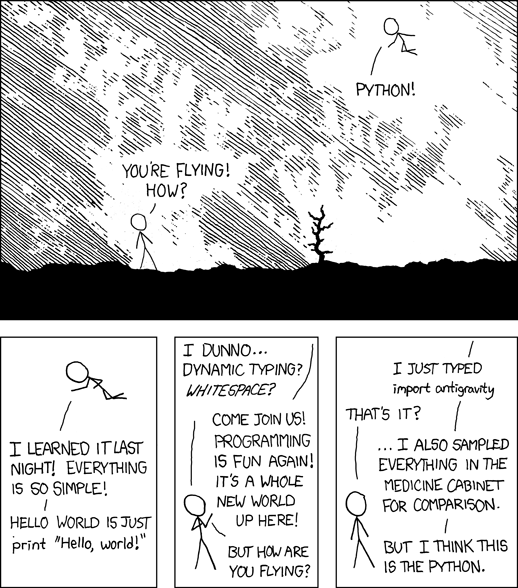
\includegraphics[height=8.3cm]{xkcd}}
    ;
    \tikz[remember picture,overlay]
      \node[anchor=south west] at (n.south east) {\tiny source: \href{http://xkcd.com/353/}{xkcd.com/353}}
    ;
\end{frame}

\begin{frame}[fragile]{Declaring Functions}
When you need a function, declare it with a \PY{k}{\tt def} statement:
\input "|./highlight.py samples/02firstprogram.py firstline=3,firstnumber=3,lastline=3"

\bigskip

Later you will need multiple arguments. Separate them with commas, like this:
\input "|./highlight.py '=def anotherFunction(a, b):' '' no"

\bigskip

Java/C++ programmers will
note that there are no type declarations: Python is a \emph{dynamically typed language}.

The types of variables are determined by what they contain.
\end{frame}

\begin{frame}[fragile]{Documenting functions}
\input "|./highlight.py samples/02firstprogram.py firstline=3,firstnumber=3,lastline=7,fontsize=!small"

In Python, you document a function by starting it with a string.

\bigskip

Use quotes to mark strings: \PY{l+s}{\tt "string"} or
\PY{l+s}{\tt \textquotesingle string\textquotesingle}.

Triple quotes (\PY{l+s}{\tt """} or \PY{l+s}{\tt \textquotesingle\textquotesingle\textquotesingle})
can be used for strings that need to span multiple lines.

\bigskip

Documentation strings, or \emph{docstrings}, should describe what a function does,
what are its arguments, and what it returns.
\end{frame}

\begin{frame}[fragile]{Indenting}
Python uses \emph{colons} and \emph{indentation} for marking code blocks, where
many other languages use \{braces\}. And it uses \emph{newlines} to separate
commands, not semicolons:

\input "|./highlight.py samples/02fact.py fontsize=!footnotesize no"

\end{frame}

\begin{frame}[fragile]{Everything is an object}
Open Python in a command line, in the directory where you saved \texttt{registration.py}, and type:

\input "|./highlight.py samples/02docsession.txt fontsize=!footnotesize"

\bigskip

1. By writing a Python file, we created an importable \emph{module}.

3. “Dot syntax” is used for \emph{attribute access}.

5. The \PY{n}{\tt\magic{doc}} attribute holds our docstring.
\end{frame}

\begin{frame}[fragile]{Testing modules}

An imported module's {\tt\magic{name}} attribute will hold the module's name:

\input "|./highlight.py samples/02namesession.txt '' no"

However, if a module is run directly, {\tt\magic{name}} will contain "\magic{main}".

This allows the following construction:

\input "|./highlight.py samples/02firstprogram.py firstline=14,firstnumber=14,lastline=14"

We use this to make sure that when imported, our program acts as a library:
it doesn't do anything, just makes a function available.

Many modules put a little functionality test in this block.

\end{frame}

\begin{frame}[fragile]{Checklist}

If managed to follow so far, you should be able to understand these:

\begin{itemize}
\item Function
\item Docstring
\item Indentation
\item Attribute
\item Module
\end{itemize}

\end{frame}

\begin{frame}[fragile]{Project}

Form teams of up to two people, and decide on what you would like to use
Python for.

\bigskip

No detailed plans at this point, just a general idea.

Send your project ideas by e-mail.


\end{frame}


\end{document}
